\documentclass[final,t]{beamer}
\mode<presentation>{
    \usetheme{cuposter}
}

% additional settings
\setbeamerfont{itemize}{size=\normalsize}
\setbeamerfont{itemize/enumerate body}{size=\normalsize}
\setbeamerfont{itemize/enumerate subbody}{size=\normalsize}
\setbeamerfont{enumerate}{size=\normalsize}
\setbeamerfont{enumerate/enumerate body}{size=\normalsize}
\setbeamerfont{enumerate/enumerate subbody}{size=\normalsize}
\beamertemplategridbackground[1.27cm]	% Display a grid to help align images

% additional packages
\usepackage{amsmath,amsthm, amssymb, latexsym}
\usepackage{cancel}
\usepackage{dsfont}
\usepackage{mathdots}
\usepackage{exscale}
\usepackage{booktabs, array}
\usepackage[english]{babel}
\usepackage[latin1]{inputenc}
\usepackage{multirow}
\usepackage[orientation=landscape,size=custom,width=101.6,height=81.28,scale=1.28]{beamerposter}
\usepackage{tikz}
\tikzset{mynode/.style={inner sep=0pt,outer sep=0pt}}
\tikzset{invisible/.style={minimum width=0mm,inner sep=0mm,outer sep=0mm}}


\usetikzlibrary{arrows,positioning}
\tikzstyle{b} = [rectangle, draw, node distance=2.5cm, text width=2em, text centered, rounded corners, minimum height=2em, thick]
\tikzstyle{l} = [draw, -latex',thick]

\tikzset{invisible/.style={minimum width=0mm,inner sep=0mm,outer sep=0mm}}
\usetikzlibrary{arrows, automata, positioning, calc}


%-------------------------------------------------------------------------------------------------
% Frame separations per columns
%-------------------------------------------------------------------------------------------------
\def\colonesep{2ex}
\def\coltwosep{.3ex}
\def\colthreesep{1.3ex}
\arraycolsep=20pt

%-------------------------------------------------------------------------------------------------
% Symbols
%-------------------------------------------------------------------------------------------------
\newcommand{\C}{\mathds{C}}
\newcommand{\D}{\mathds{D}}
\newcommand{\N}{\mathds{N}}
\newcommand{\R}{\mathds{R}}

\title{\huge Flu Forecasting using Climate Data and Bayesian Hierarchical Modeling}
\author[]{\Large Maia Richards-Dinger$^1$ and Dr. Stephen Kissler$^2$ \\
\small$^1$CU Boulder - Applied Math Department, $^2$CU Computer Science Department}

%\institute[]{Department of Mathematics, Department of Biology, University of Wisconsin-La Crosse}
%\date[Aug. 10 , 2019]{Aug. 31 , 2019}

%-------------------------------------------------------------------------------------------------
\begin{document}
\begin{frame}{}
	\begin{columns}[t]
		\begin{column}{.31\linewidth}
			%!TEX root = ../march2025poster.tex

\begin{block}{Motivation and Background}
	
\textbf{Importance of Forecasting}
\begin{itemize}
	\item Influenza places a significant disease burden on temperate countries in the Northern Hemisphere every winter
	\item Accurate forecasts can help hospitals prepare for spikes and decide how to ration medication, and can impact how individuals make decisions regarding vaccination, mask wearing, travel, etc.
\end{itemize}
	
\textbf{Original motivating questions}
	\begin{itemize}
		\item How do scoring rules (explicit or implicit) potentially impact infectious disease forecasting competition submissions?
		\begin{itemize}
			\item[$\cdot$] Frongillo [3] studied how improper scoring rules can incentivize forecasters to report predictions that do not align with their true beliefs - could this be affecting the submissions to disease forecasting competitions?
		\end{itemize}
	\item CDC organizes the FluSight competition and uses the multibin logarithmic scoring rule, which is not proper [1]
		\item What is the optimal way to aggregate ensemble forecasts? 
		\begin{itemize}
			\item[$\cdot$] CDC currently seems to just take the median
		\end{itemize}
	\end{itemize}	

\textbf{Currect Project}
\begin{itemize}
	\item Goal: Forecast flu incidence at the state level using climate data
	\item Cold and dry conditions have been shown to correlate with increased flu (and other respiratory infection) activity [2]
	\item  Can incorporating climate data improve flu forecasts? 
\end{itemize}
\end{block}

\vspace{\colonesep}

\begin{block}{Methods}
\textbf{Step 1: Calculate ILI plus}
\begin{itemize}
	\item CDC collects data on percent of healthcare visits due to influenza-like illness (ILI) by state and publishes it weekly
	\item Report percent of flu tests that are positive by state each week
	\item As in Goldstein et al. [4], we use the product of percent visits due to ILI and percent positive flu tests as a proxy for flu incidence, which we call ILI plus
\end{itemize}

\textbf{Step 2: Fit a piecewise linear functions}
\begin{itemize}
	\item Since we expect flu incidence to grow and decay exponentially, we expect the log of ILI plus to grow and decay linearly
	\item For each flu season and state, fit a piecewise linear function with two breaks to the log of ILI plus data
	\item Record up slope, down slope, peak week, and peak value
\end{itemize}
\begin{center}
	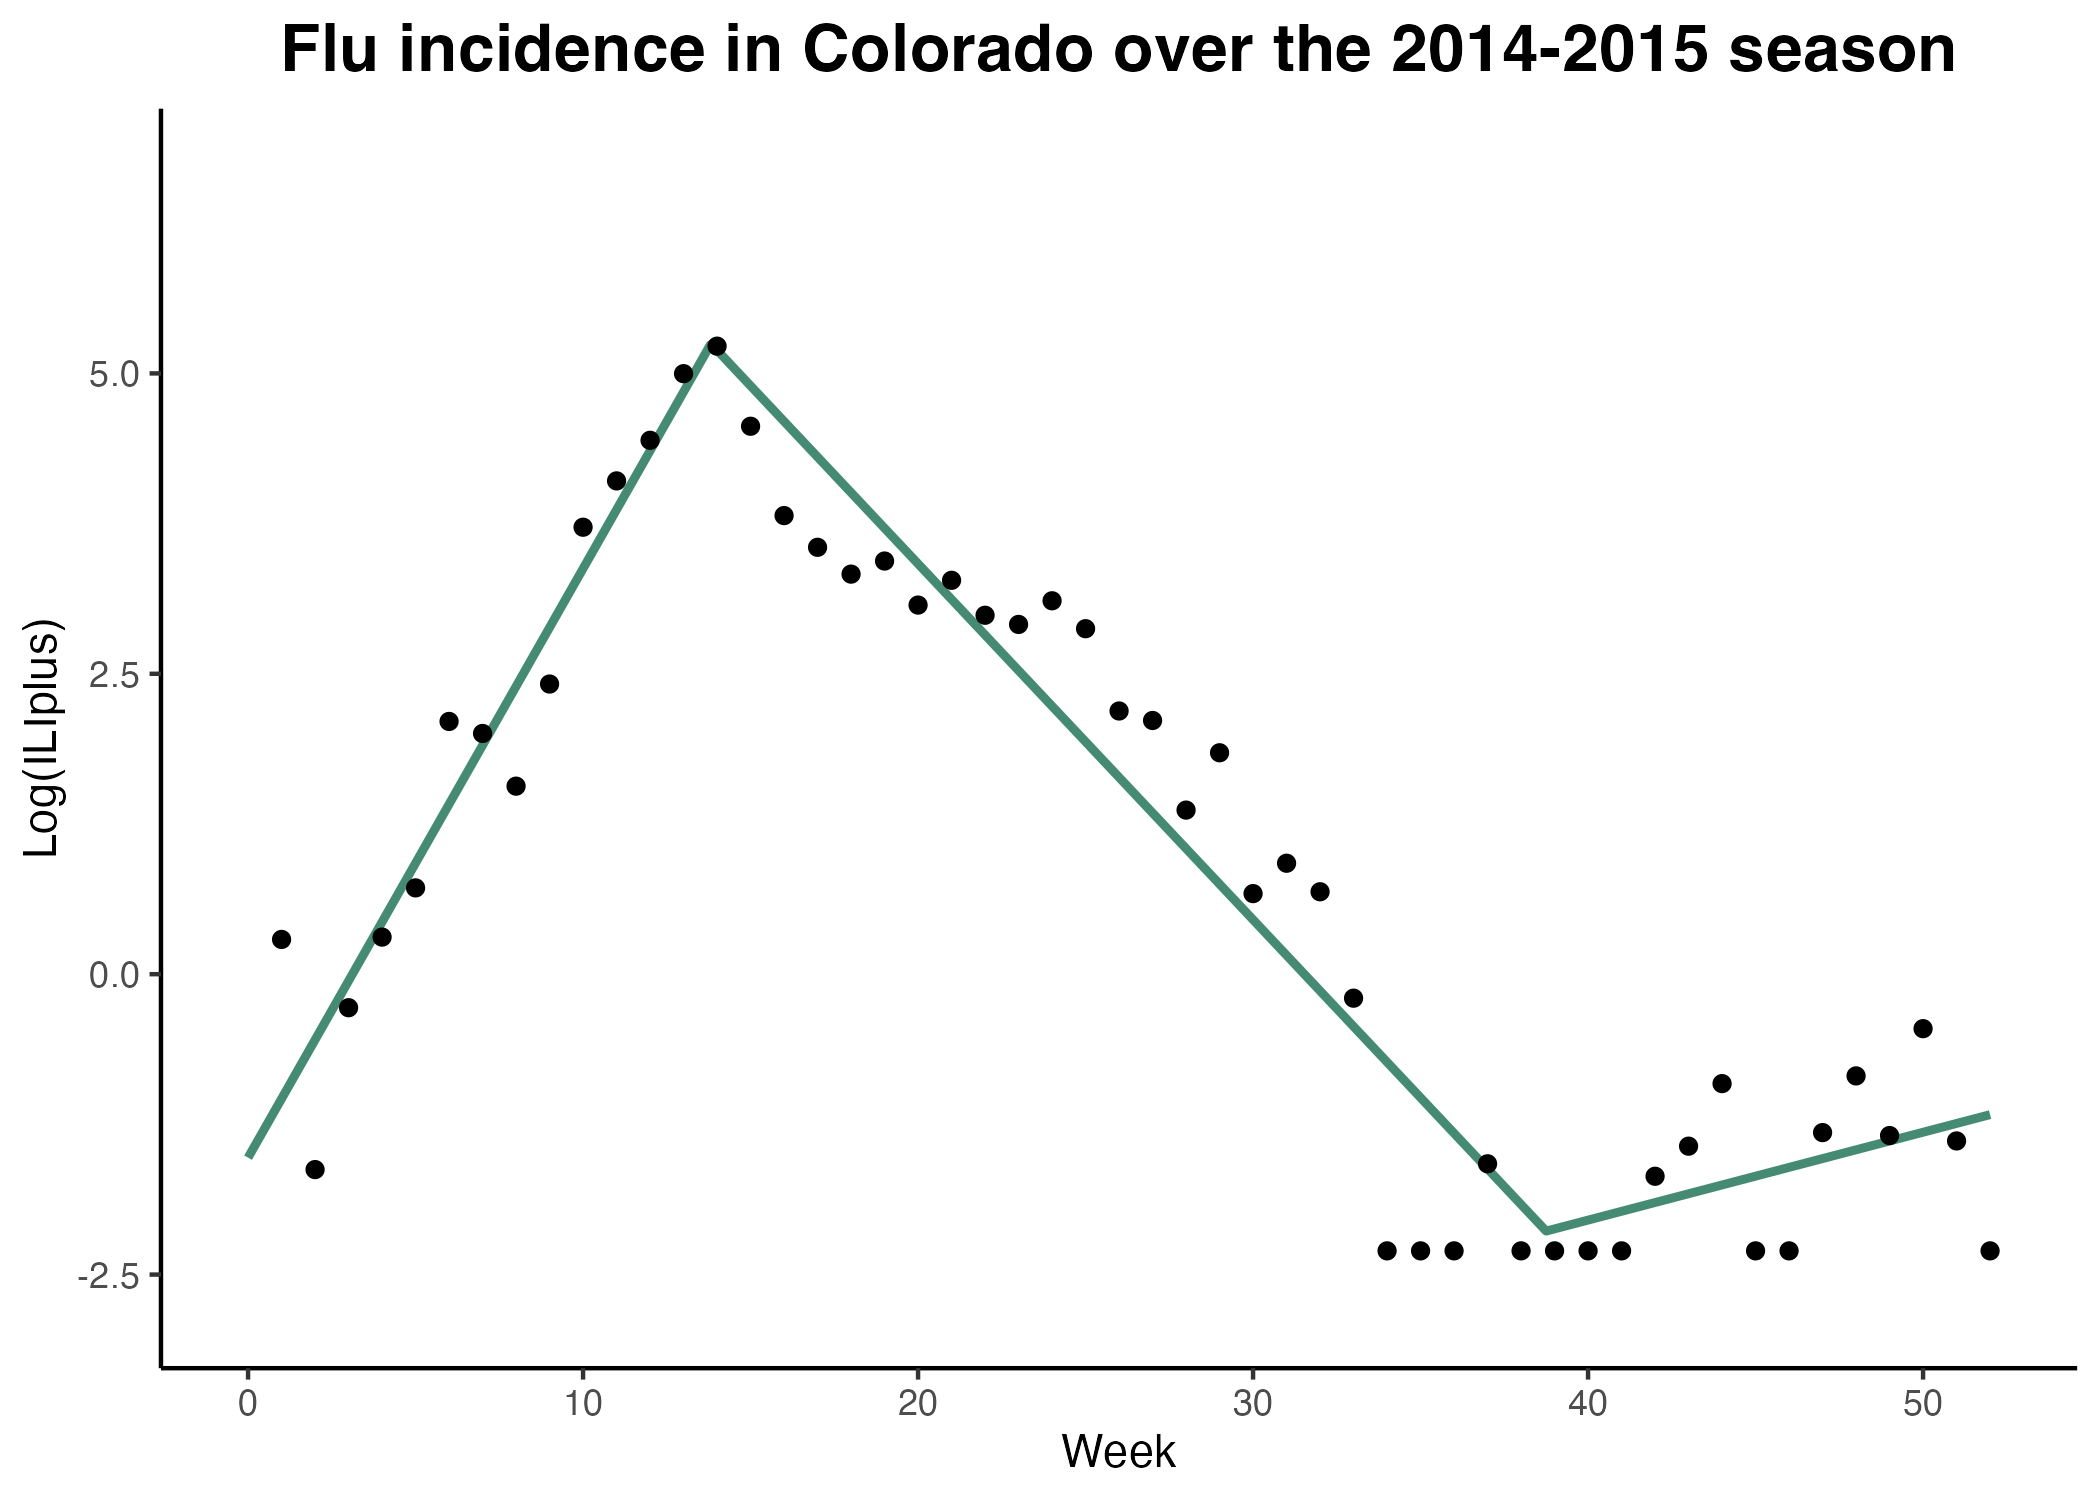
\includegraphics[width = 0.59\columnwidth]{sections/images/Colorado2014(just-fit).png}
\end{center}
\end{block}

		\end{column}
        
		\begin{column}{.3\linewidth}
			%!TEX root = ../march2025poster.tex

\begin{block}{Methods (cont.)}
\textbf{Step 3: Predict parameters using climate and population data}
\begin{itemize}
	\item Calculate the population density ($x_1$), percent of people under 18 ($x_2$), latitude ($x_3$), mean maximum temperature ($x_4$), mean maximum relative humidity ($x_5$), mean minimum relative humidity ($x_6$), and mean average absolute humidity ($x_7$) for each state and flu season, using census population data and gridMET climate data 
	\item Use Monte Carlo Markov Chain methods in Stan to fit the following statistical model $$y_k \sim \alpha_k + \sum_{i=1}^7 \beta_{ik}x_i + \text{Normal}(0, \sigma_k)$$ for $k = 1,2,3,4$, where $y_1=$ up slope, $y_2=$ down slope, $y_3=$ peak week, and $y_4=$ peak value
	\item Use $\alpha_k$ and $\beta_{ik}$ to predict the piecewise linear fit for each flu season and state based on the climate and population variables for that season/state and compare to the actual fit
\end{itemize}	

\end{block}

\vspace{\coltwosep}

\begin{block}{Results (so far)}
	\begin{center}
		\begin{figure}
			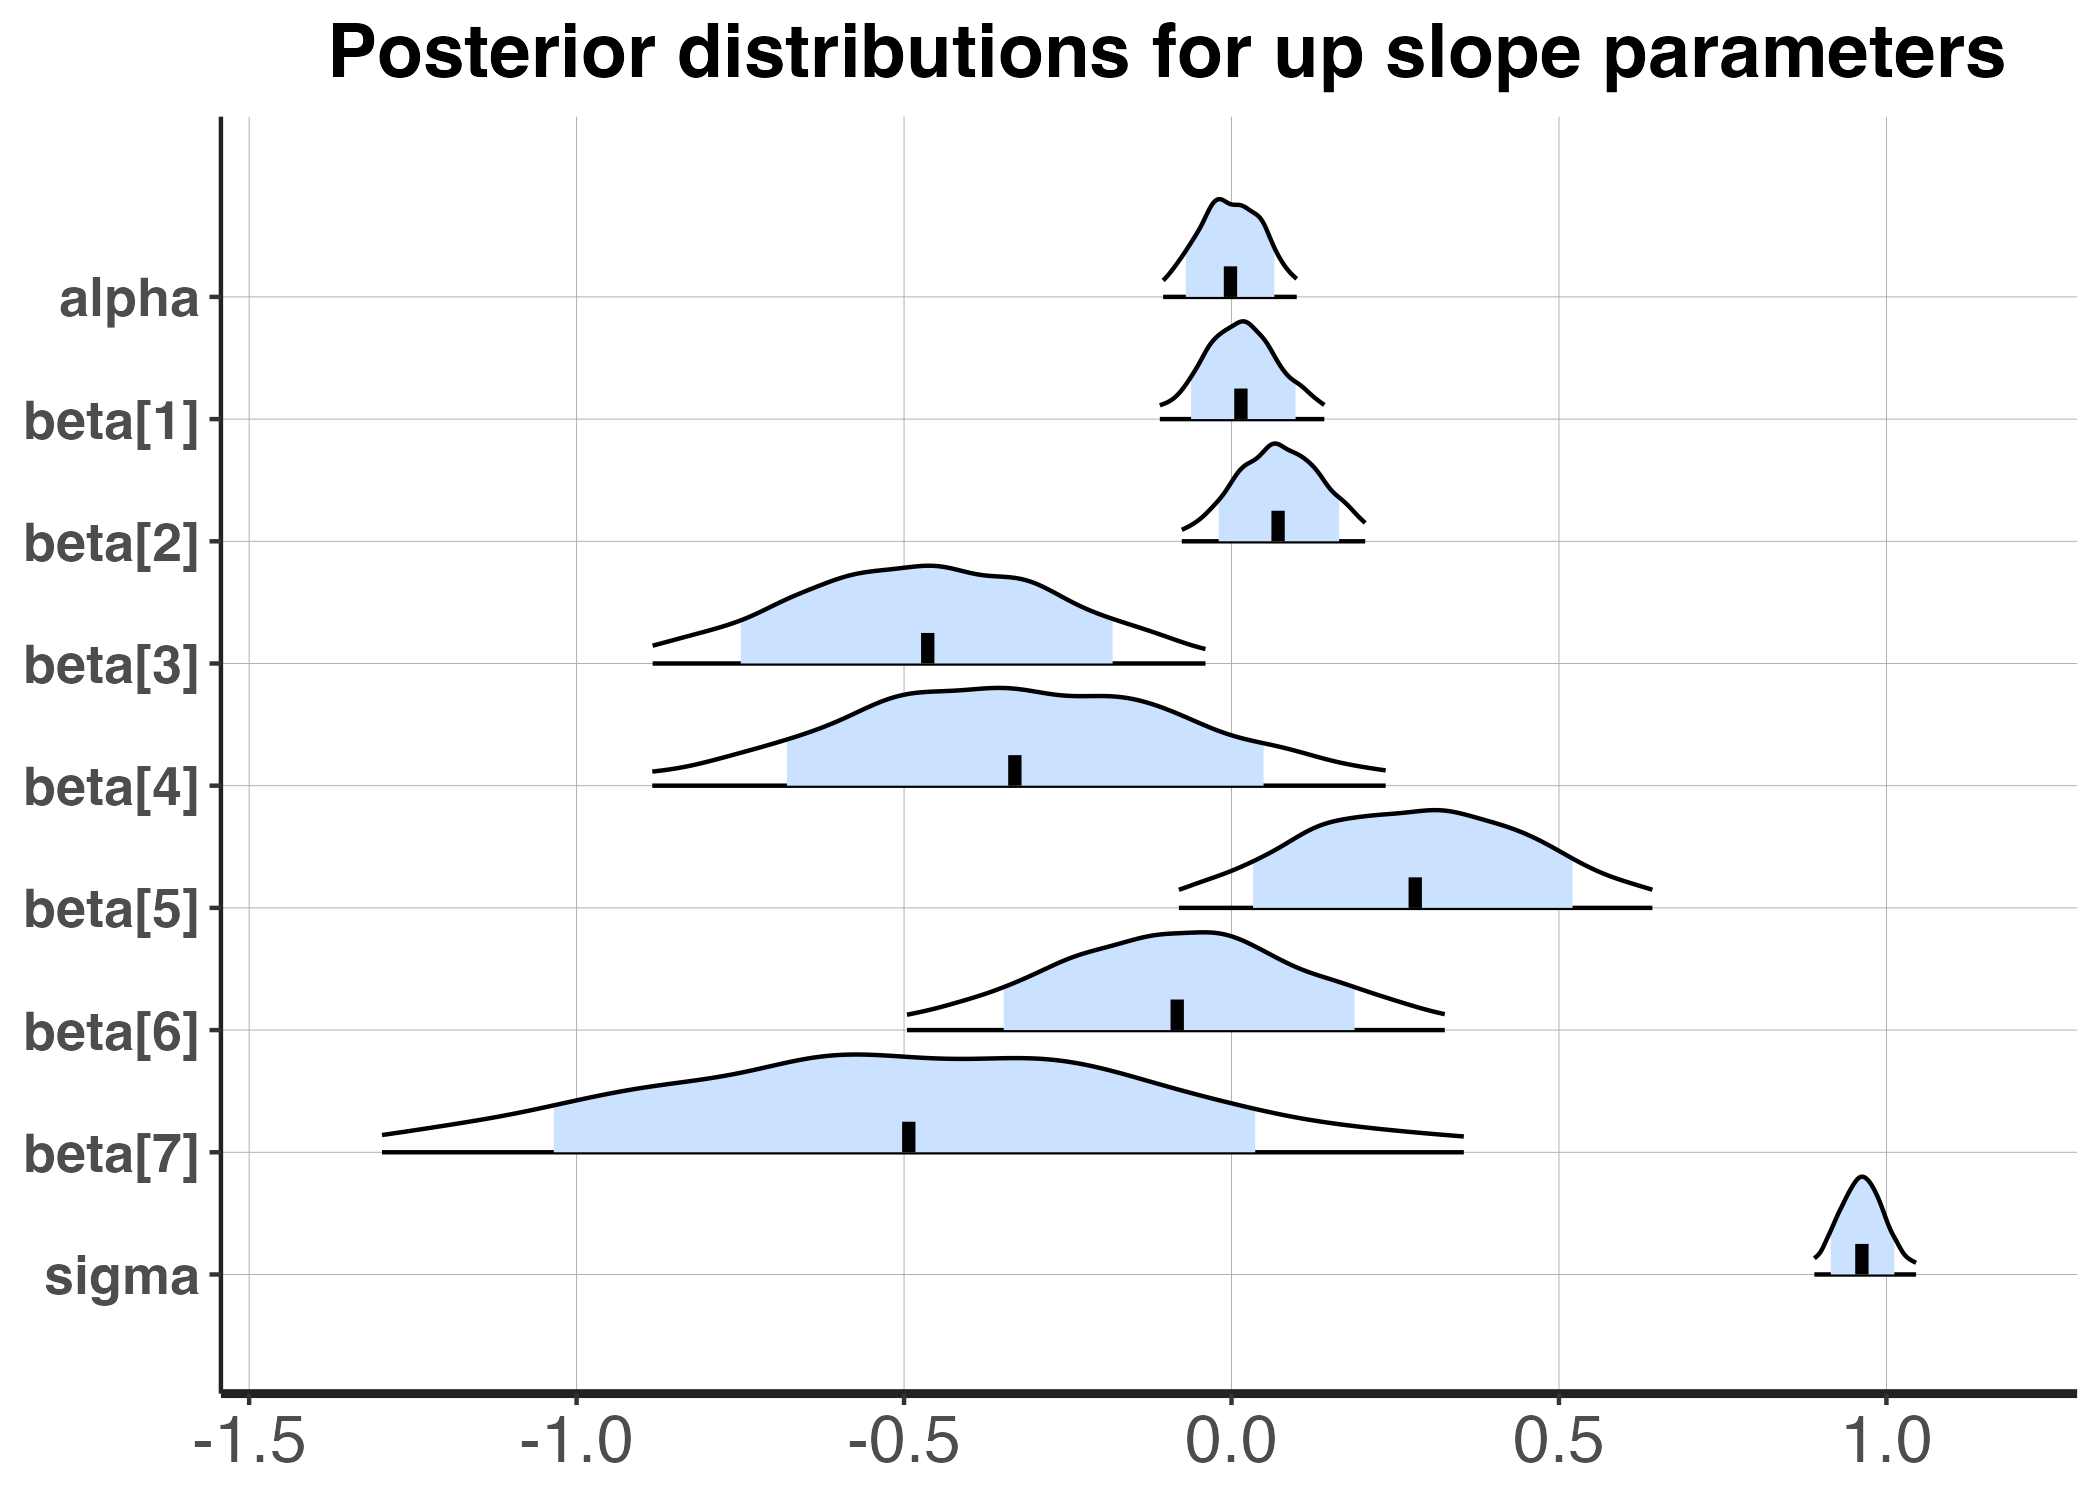
\includegraphics[width = 0.48\columnwidth]{sections/images/upslope_plot.png}
			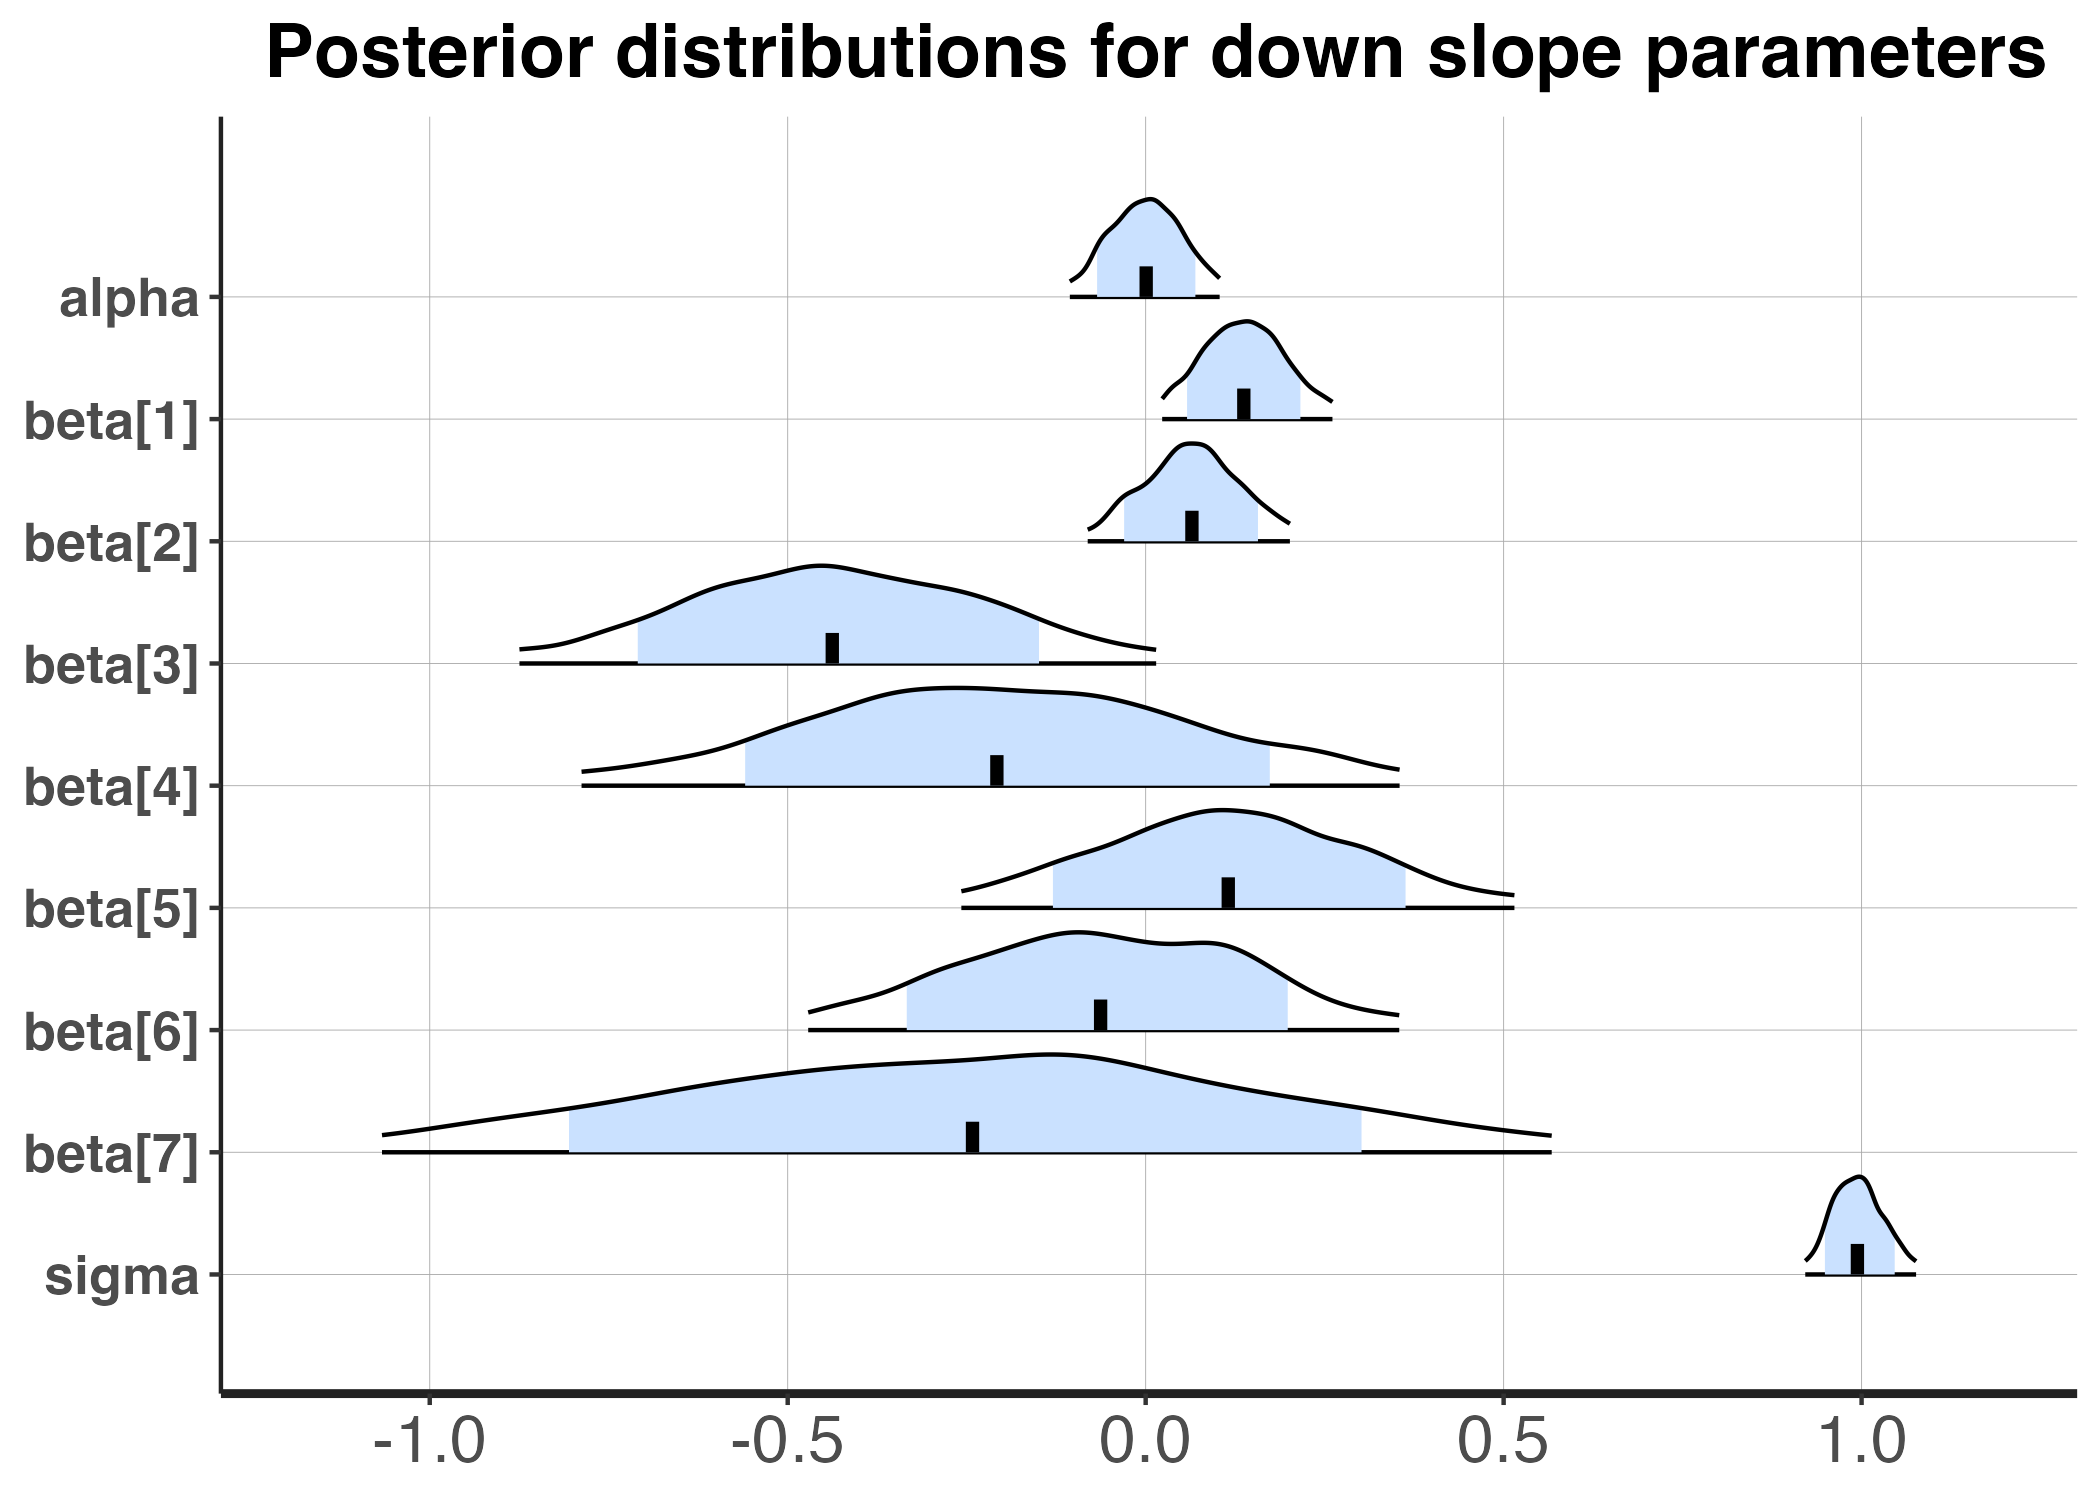
\includegraphics[width = 0.48\columnwidth]{sections/images/downslope_plot.png}
			\\
			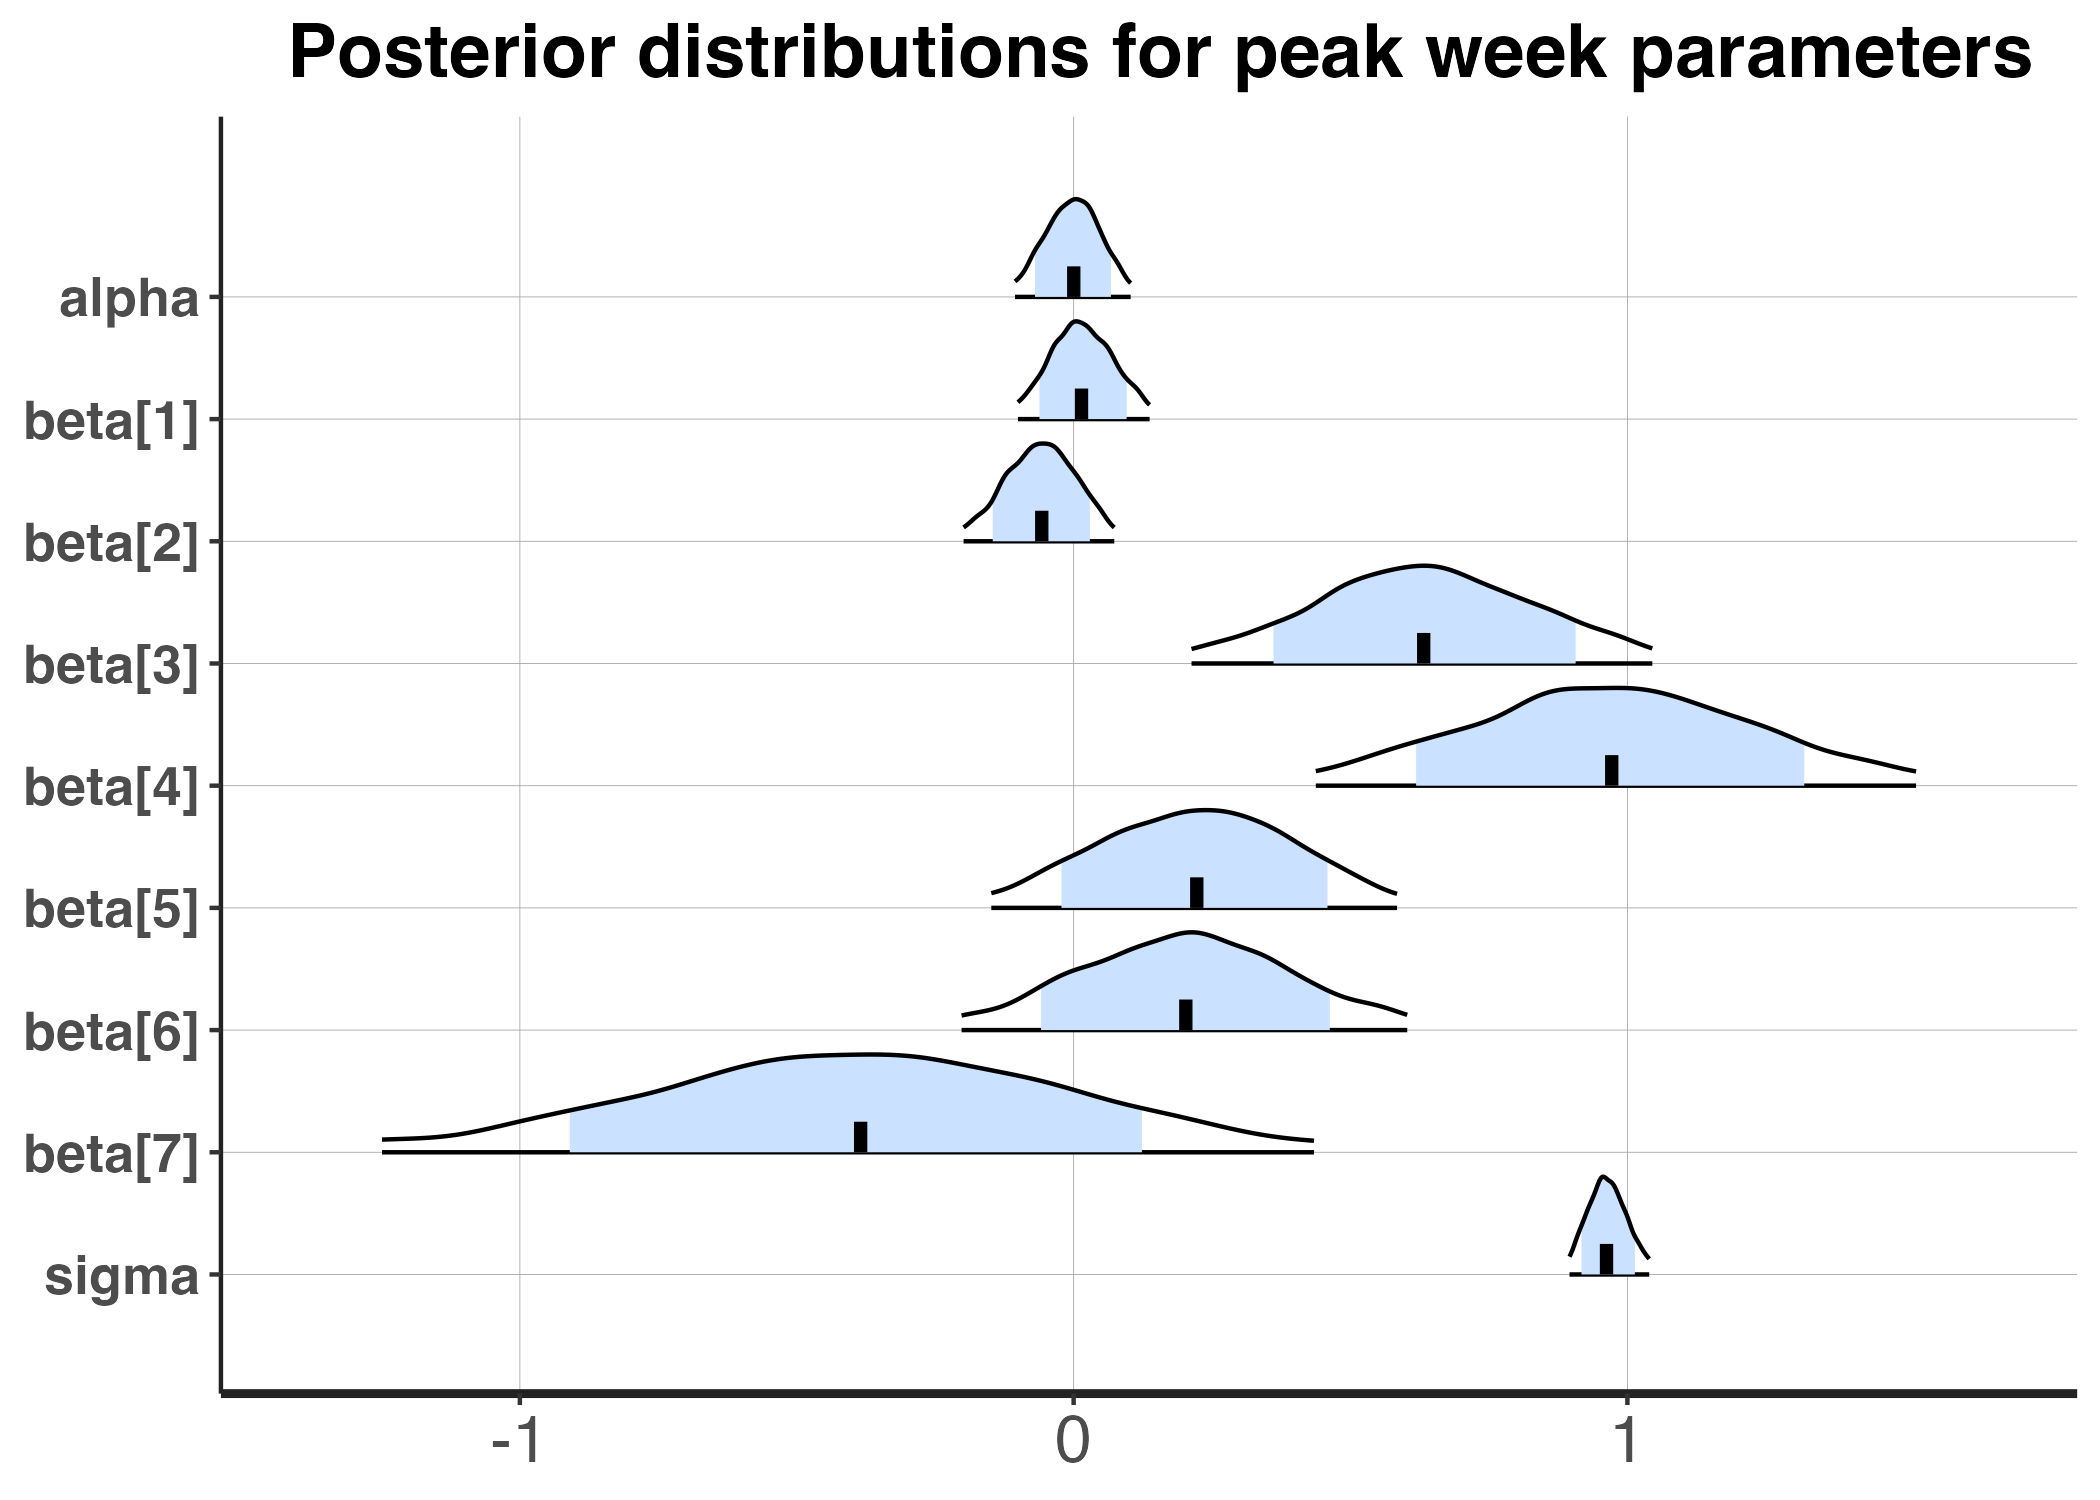
\includegraphics[width = 0.48\columnwidth]{sections/images/peakwk_plot.png}
			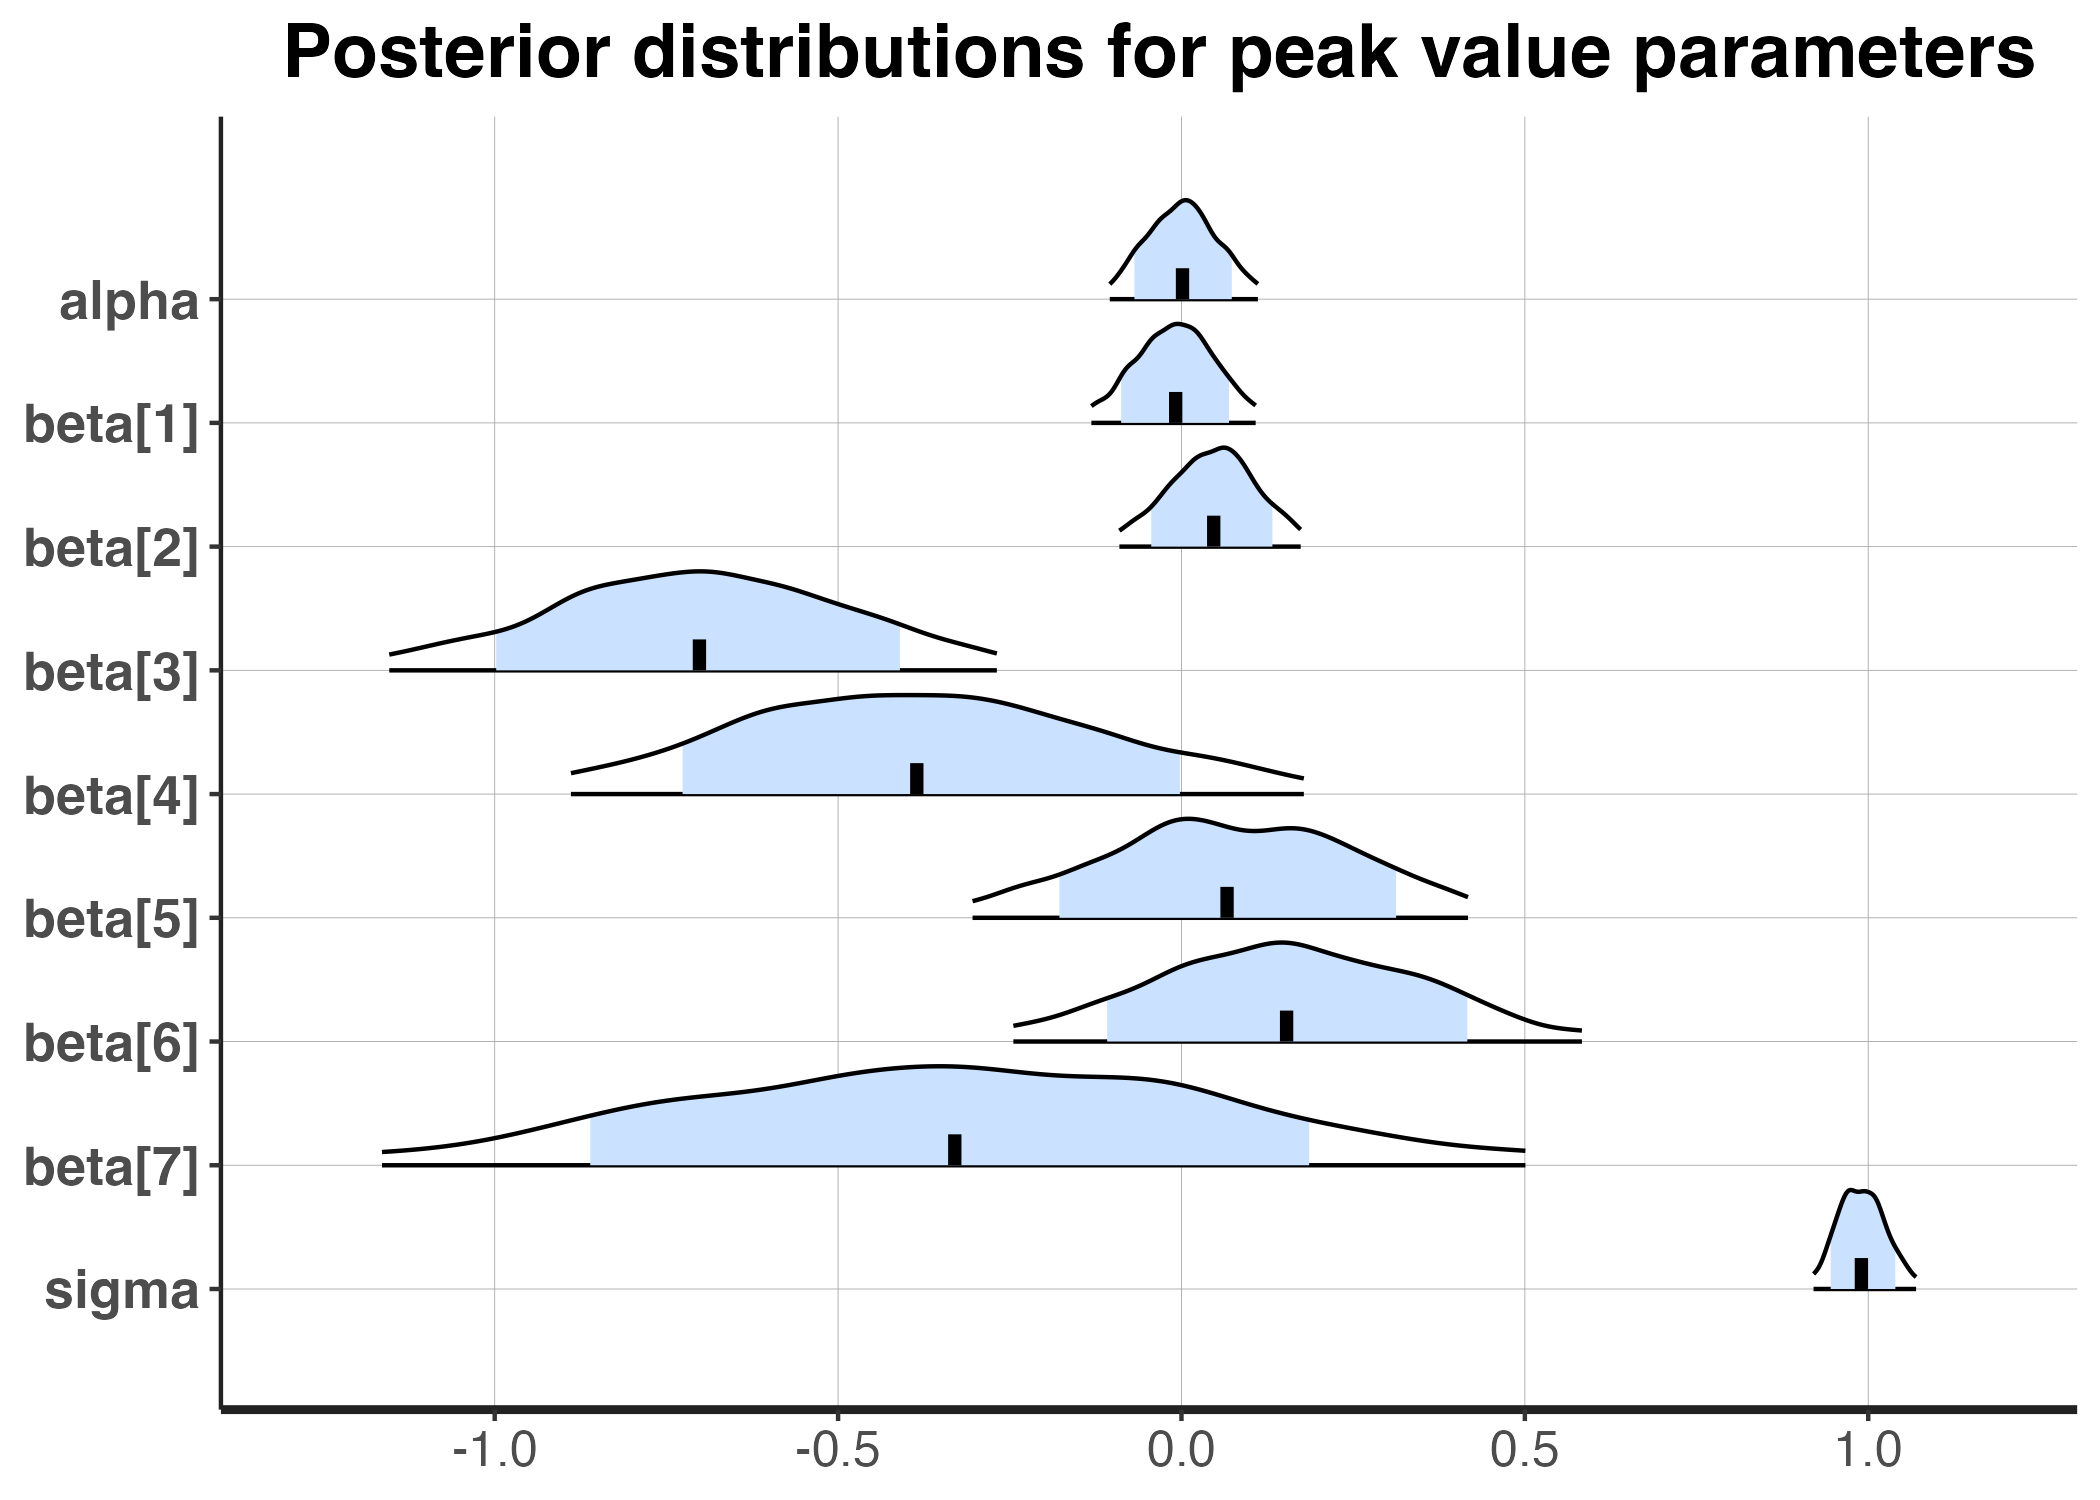
\includegraphics[width = 0.48\columnwidth]{sections/images/peakval_plot.png}\\
			\caption{Posterior distributions for $\alpha_k, \beta_{ik}, \sigma_k$ parameters for up slope, down slope, peak week, and peak value. The blue shaded regions are $80\%$ credible intervals and the total lines plotted are $95 \%$ credible intervals.}
		\end{figure}
	\begin{itemize}
		\item Overall $\beta_3$, which corresponds to latitude, is the most significant
		\item The further north a state is, the less steep their up slope tends to be, the steeper their down slope tends to be, the later their peak week tends to be, and the smaller their peak value tends to be
		\item The more dense a state is, the less steep their down slope tends to be
		\item The hotter a state is in a given year, the later their peak week tends to be
	\end{itemize}
	\end{center}

\end{block}


		\end{column}
		
		\begin{column}{.3\linewidth}
			%!TEX root = ../march2025poster.tex

\begin{block}{Results so far (cont.)}
\begin{center}
	\begin{figure}
		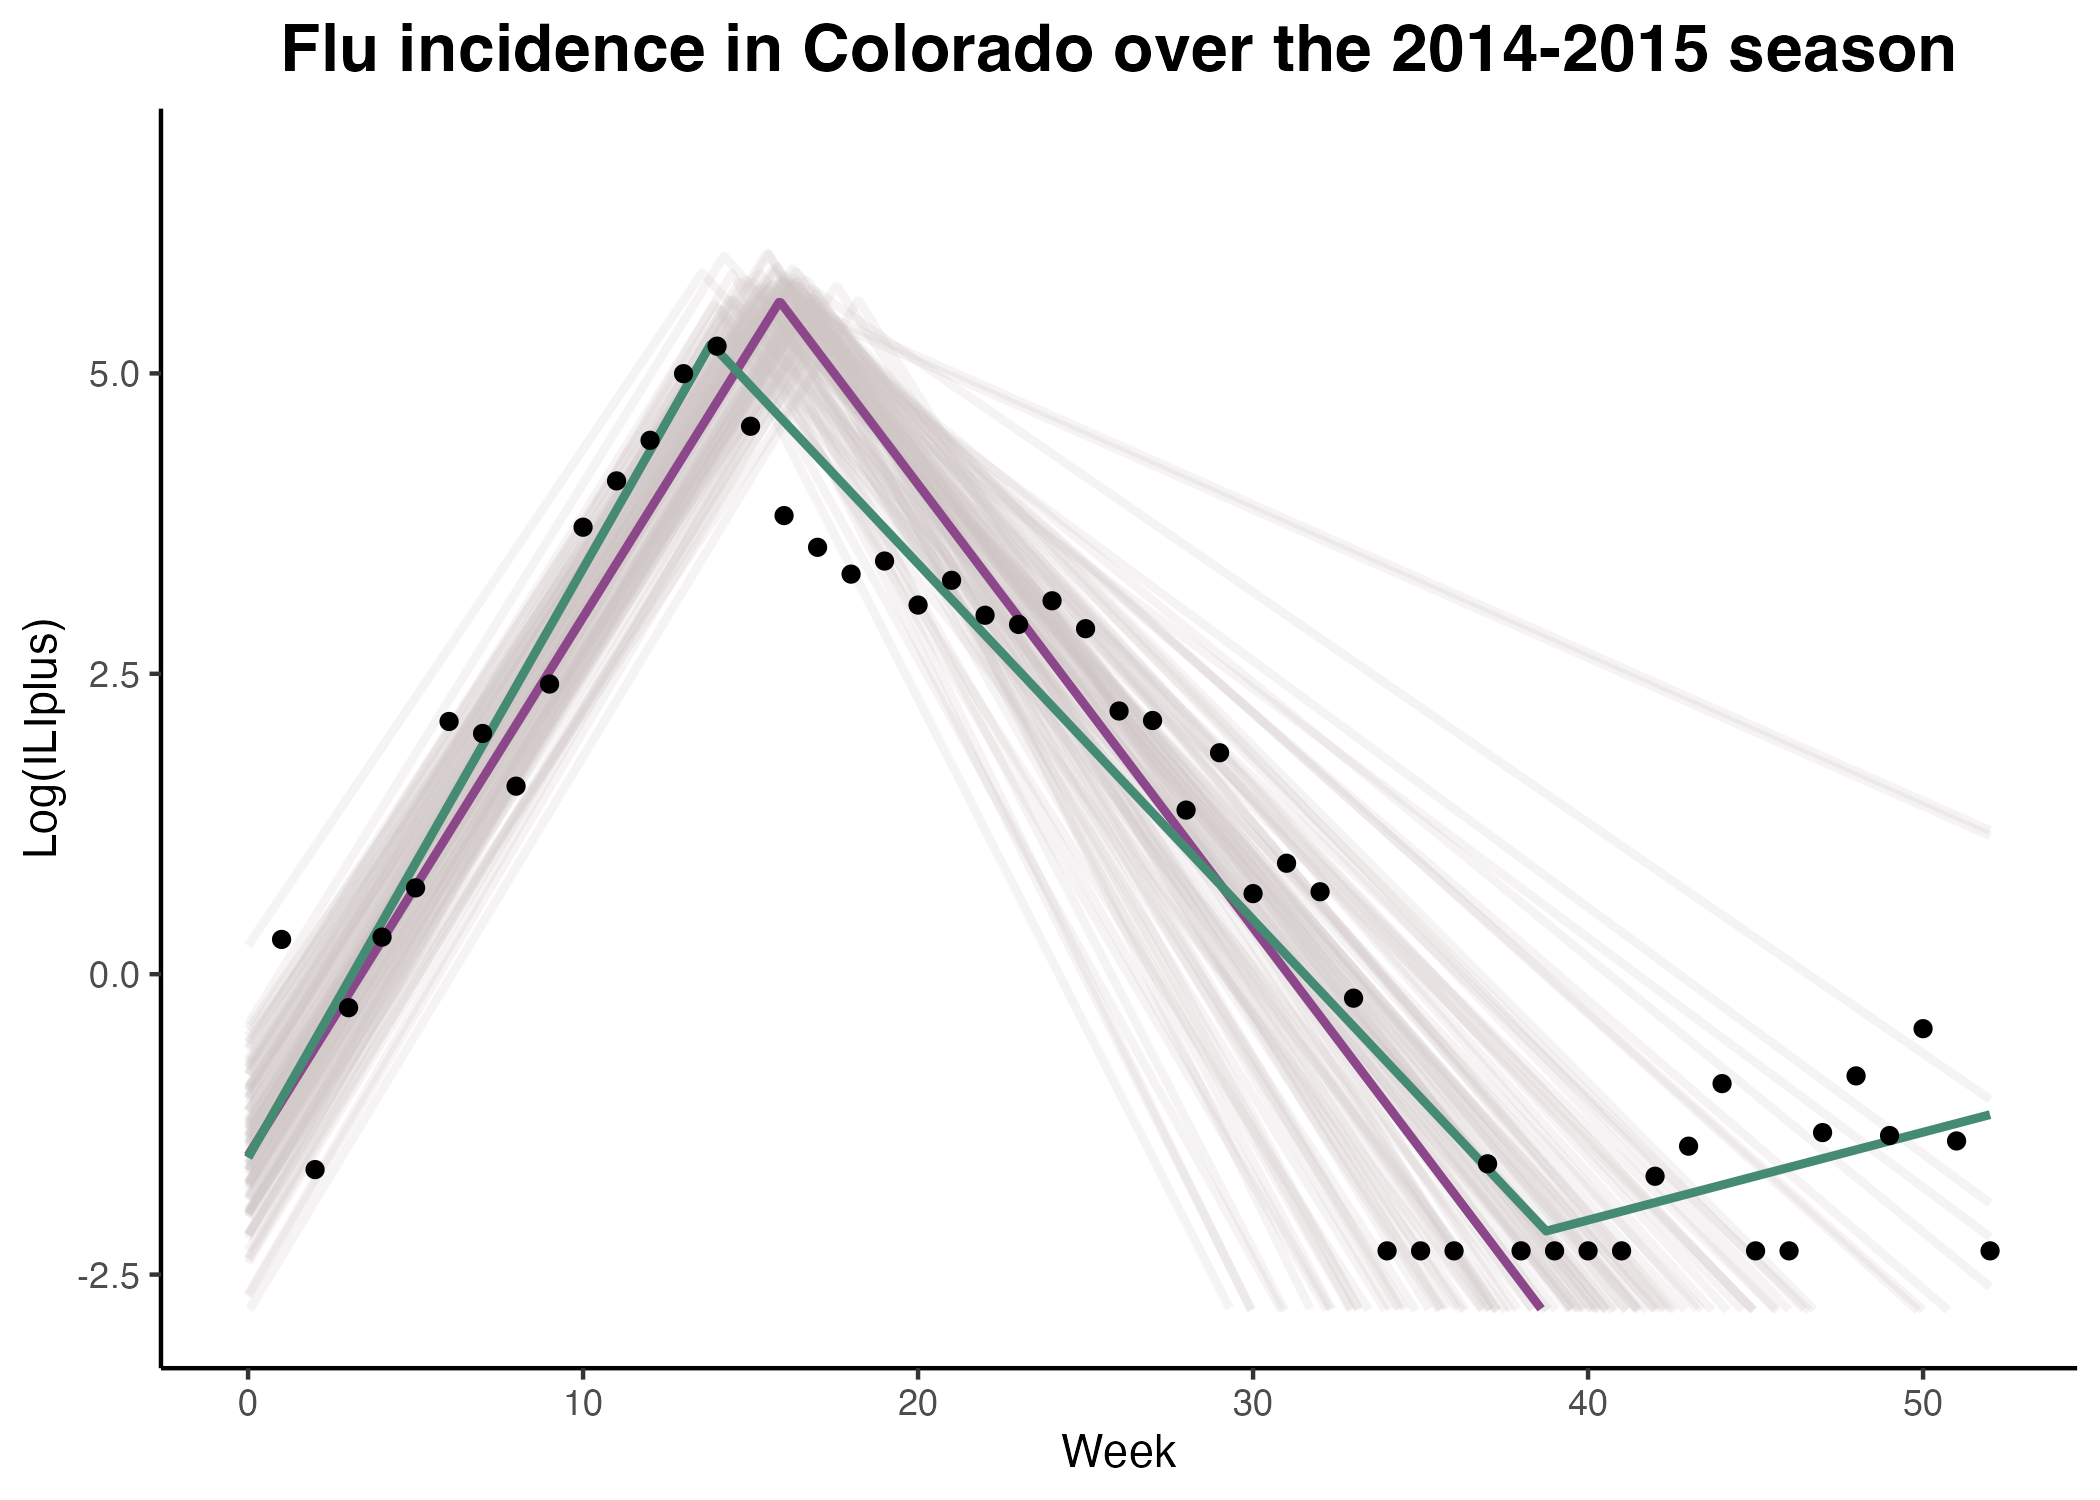
\includegraphics[width = 0.48\columnwidth]{sections/images/Colorado2014.png}
		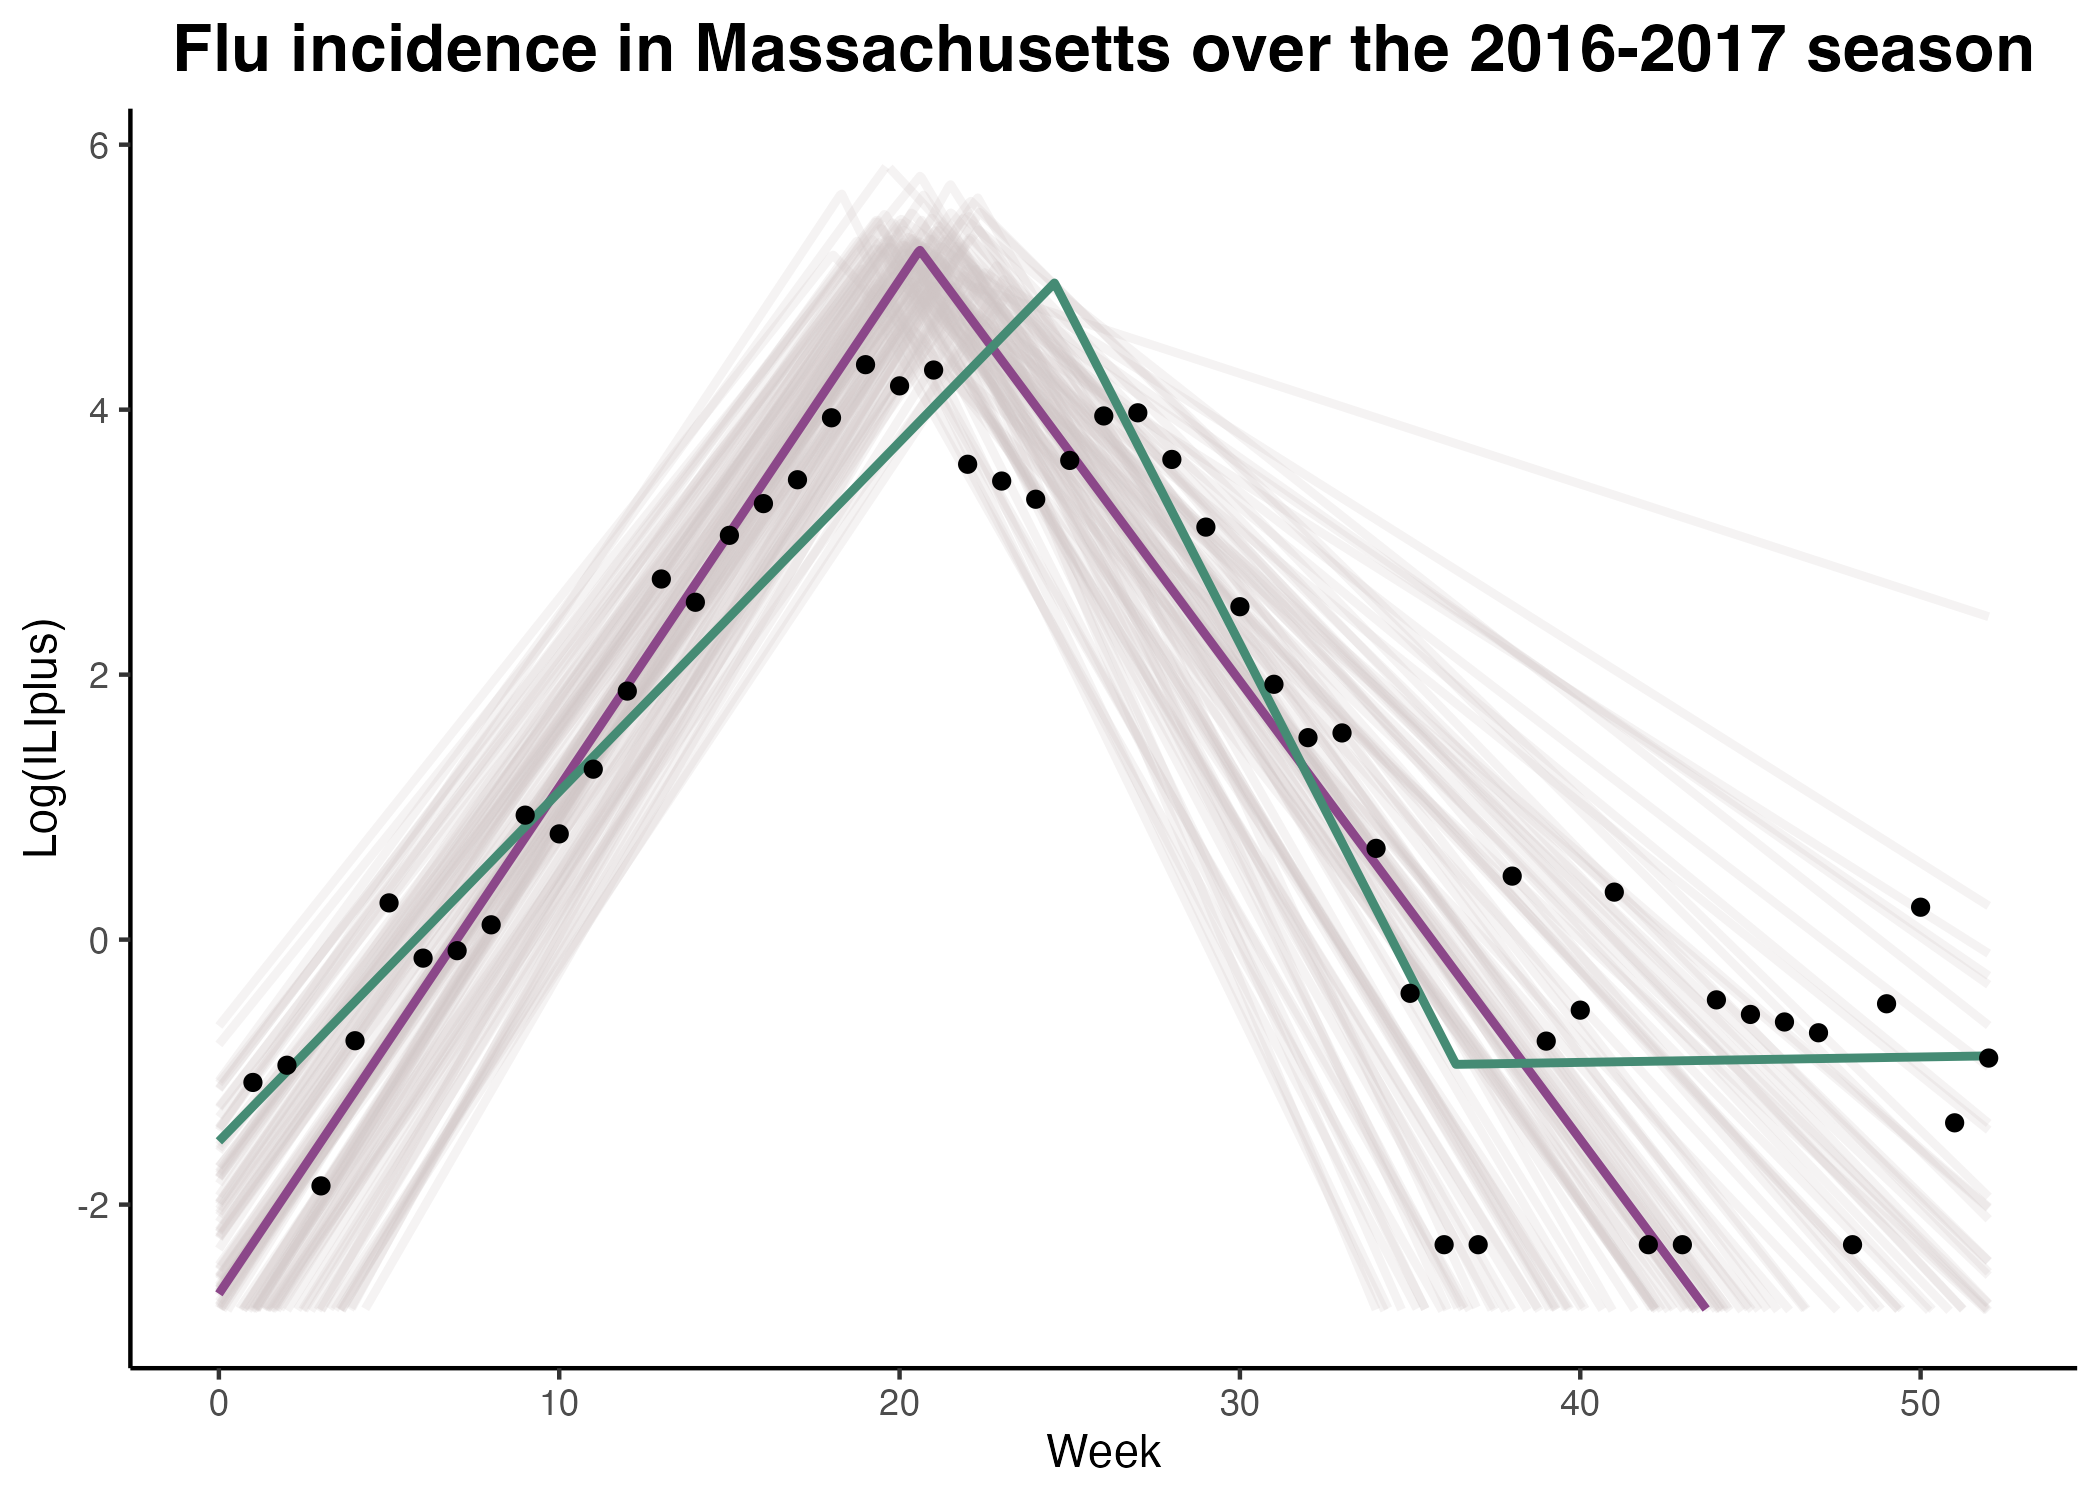
\includegraphics[width = 0.48\columnwidth]{sections/images/Massachusetts2016.png}
		\\
		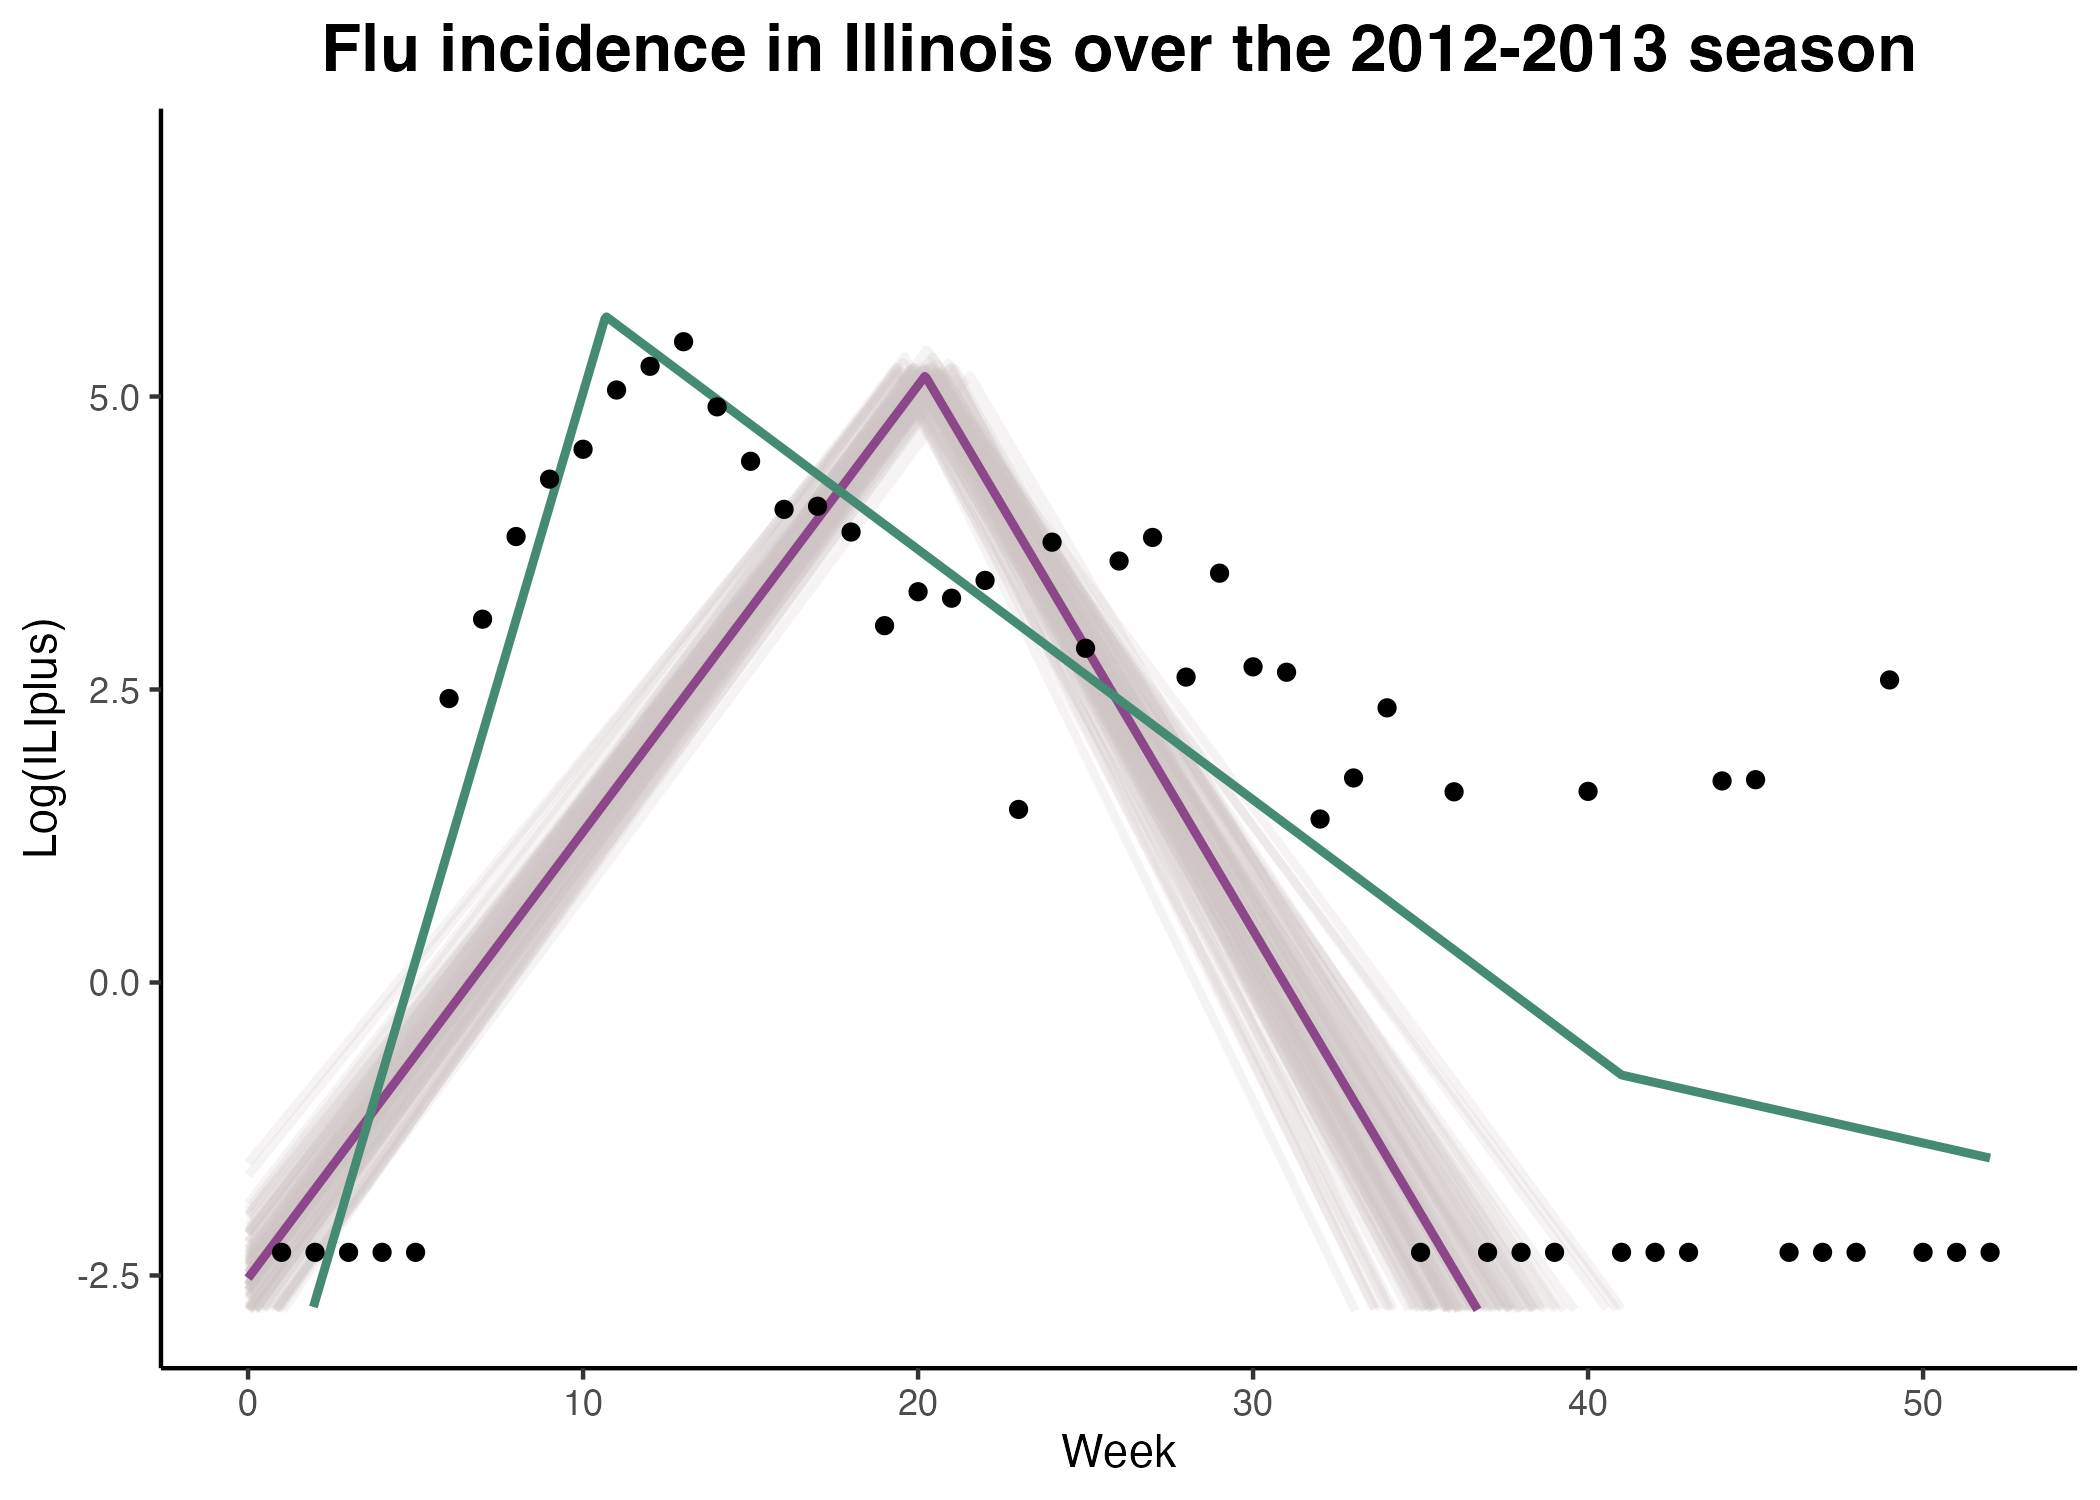
\includegraphics[width = 0.48\columnwidth]{sections/images/Illinois2012.png}
		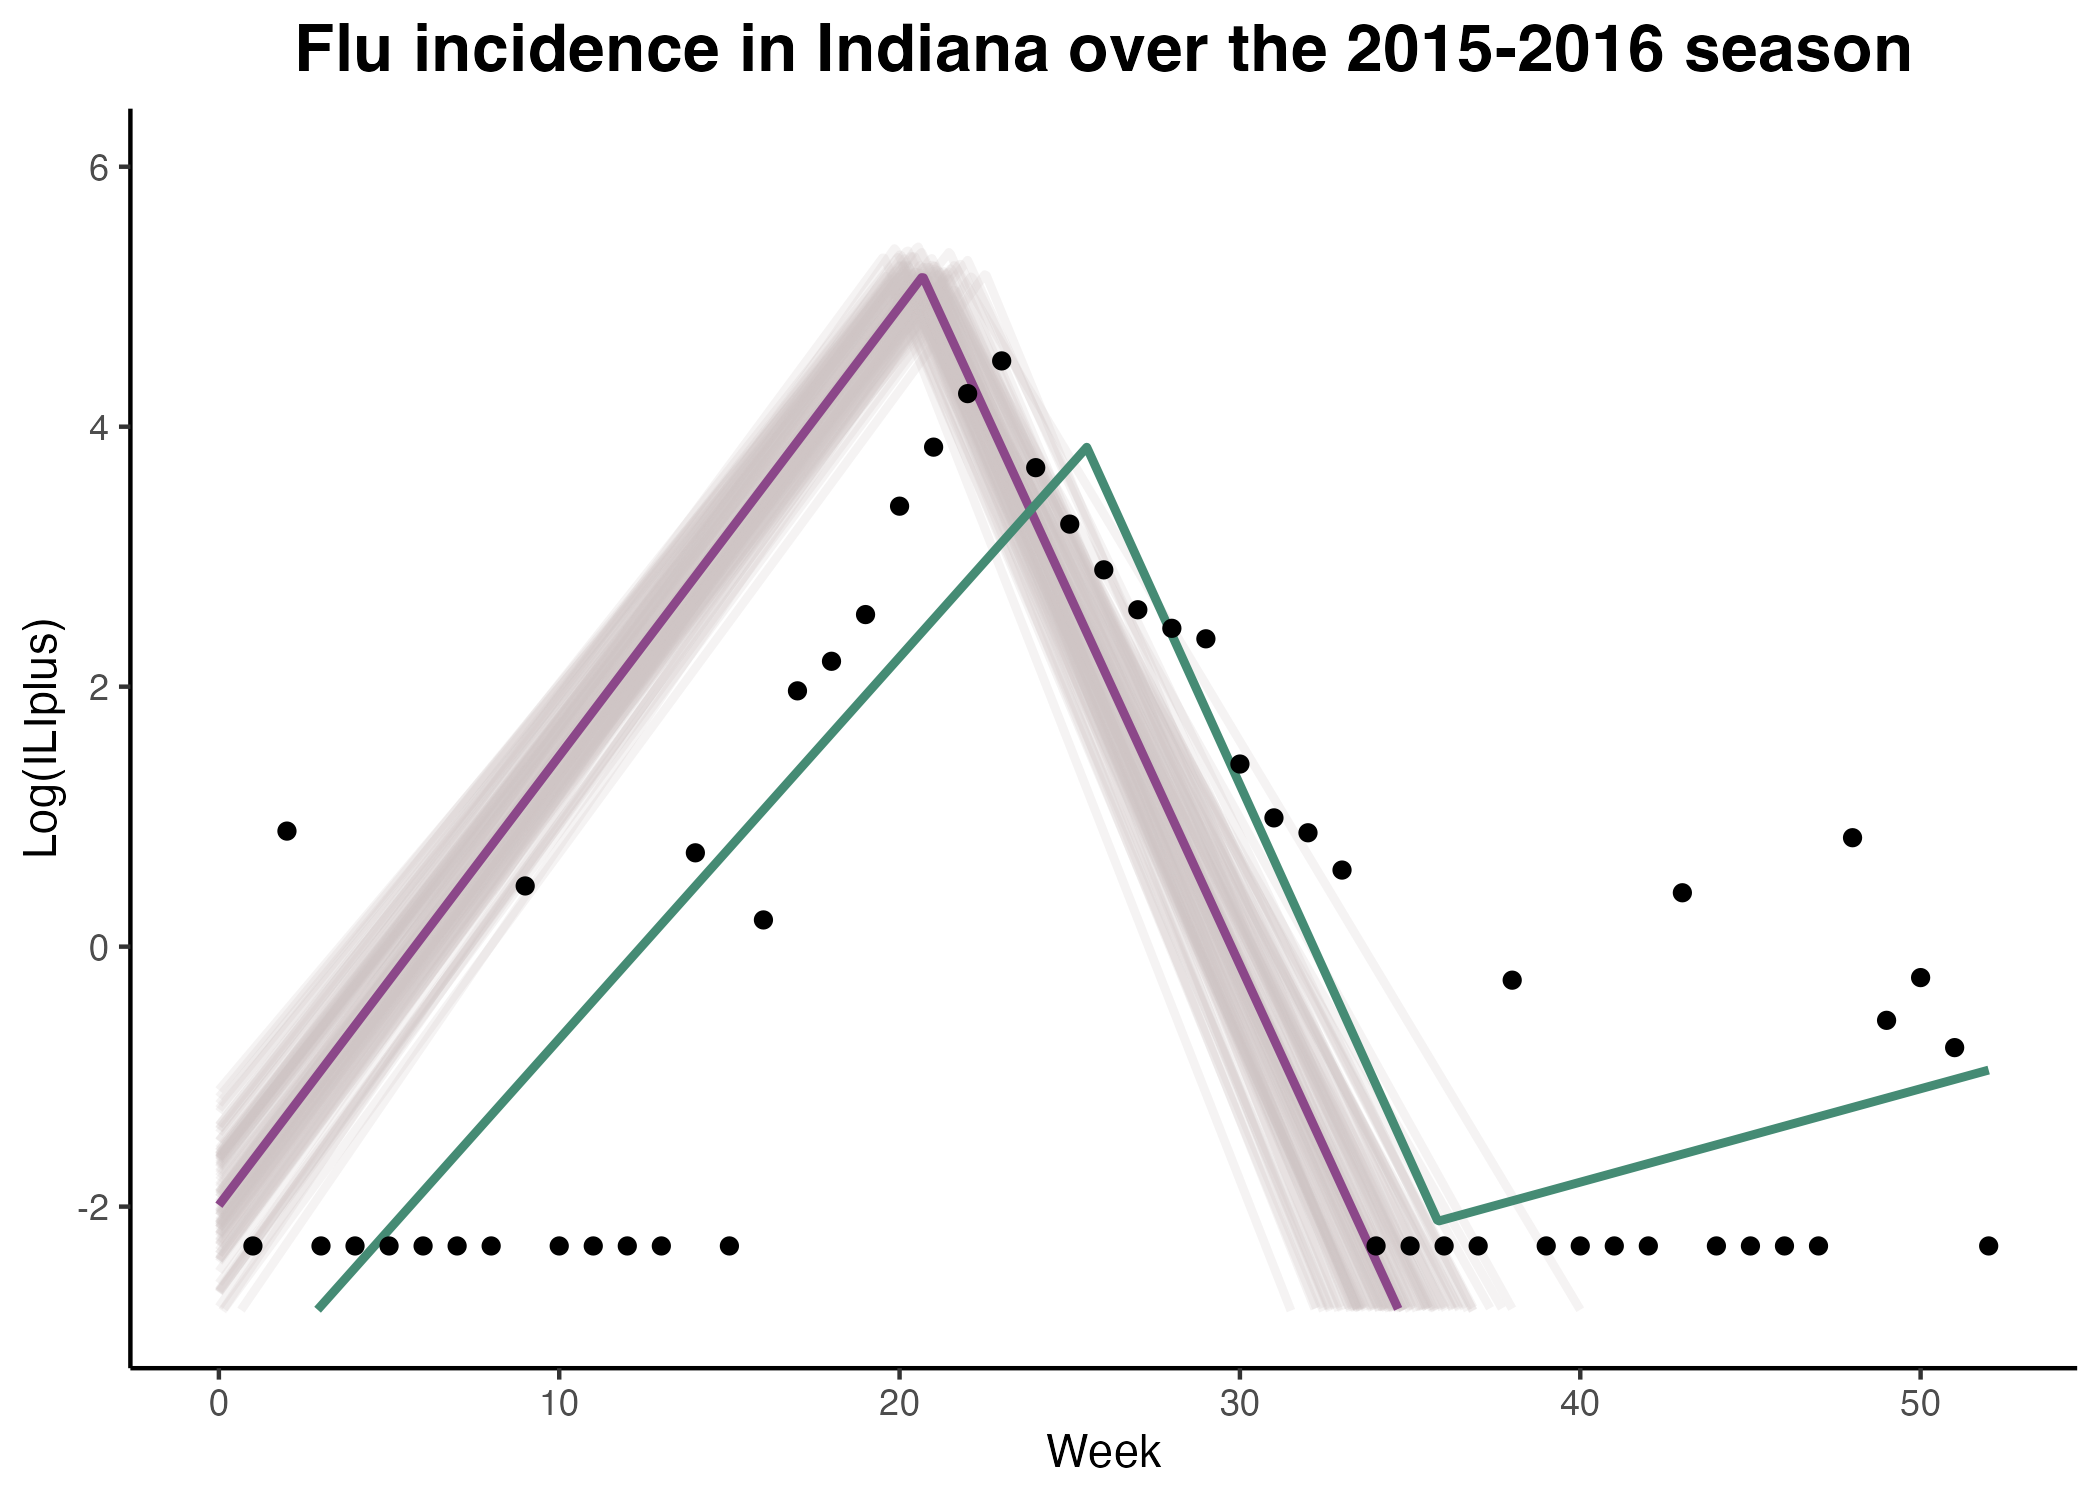
\includegraphics[width = 0.48\columnwidth]{sections/images/Indiana2015.png}\\
		\caption{Flu incidence in four different states and years along with the piecewise linear fit (green line) and the piecewise linear fits predicted by that state/year's climate and population data (mean of posterior distribution - purple line, 100 draws from posterior distribution - light purple lines).}
	\end{figure}
\end{center}
\begin{itemize}
	\item Some predicted fits are quite good! 
	\item Others are not as good
	\item In general, the Bayesian model parameter predictions have less variance than the true parameters (up slope, down slope, etc.)
\end{itemize}
\end{block}
\vspace{\colthreesep}

\begin{block}{Future Work}
	\begin{itemize}
		\item Consider other climate variables (e.g. minimum temperature) and timing of climate variables (i.e. we'd expect the temperature, humidity, etc. earlier in the season to have a greater impact)
		\item Model evaluation and comparison 
		\item Implement Bayesian *hierarchical* modeling
		\item Actually create forecasts using an ARIMA (autoregressive integrated moving average) model 
	\end{itemize}
\end{block}

\vspace{\colthreesep}

\begin{block}{References}
	\leftskip 01in
	\parindent -01in
	[1] Bracher, Johannes. "On the multibin logarithmic score used in the FluSight competitions."\textit{ Proceedings of the National Academy of Sciences} 116.42 (2019): 20809-20810. \\
	\vspace{.75ex}
	[2] du Prel, Jean-Baptist, et al. "Are meteorological parameters associated with acute respiratory tract infections?." \textit{Clinical infectious diseases} 49.6 (2009): 861-868. \\
	\vspace{.75ex}
	[3] Frongillo, Rafael M. \textit{Eliciting private information from selfish agents}. University of California, Berkeley, 2013. \\
	\vspace{.75ex}
	[4] Goldstein, Edward, et al. "Predicting the epidemic sizes of influenza A/H1N1, A/H3N2, and B: a statistical method." \textit{PLoS medicine} 8.7 (2011): e1001051. 

\end{block}

 
		\end{column}
	\end{columns}   
\end{frame}
\end{document}